\documentclass[tikz,border=12pt]{standalone}
\usepackage[T1]{fontenc}
\usepackage{mathpazo}
\usepackage{amsmath,amssymb}
\usetikzlibrary{arrows.meta, calc}

\definecolor{stblue}{HTML}{7B97AD}
\definecolor{rwgold}{HTML}{B8995E}
\definecolor{sage}{HTML}{7A9A7E}
\definecolor{dkbrown}{HTML}{3D3530}
\definecolor{wmgray}{HTML}{7B7067}
\definecolor{cream}{HTML}{F9F6F0}
\definecolor{border}{HTML}{D4C9B8}
\definecolor{terracotta}{HTML}{C47A6A}
\definecolor{lavender}{HTML}{907EA0}

\begin{document}
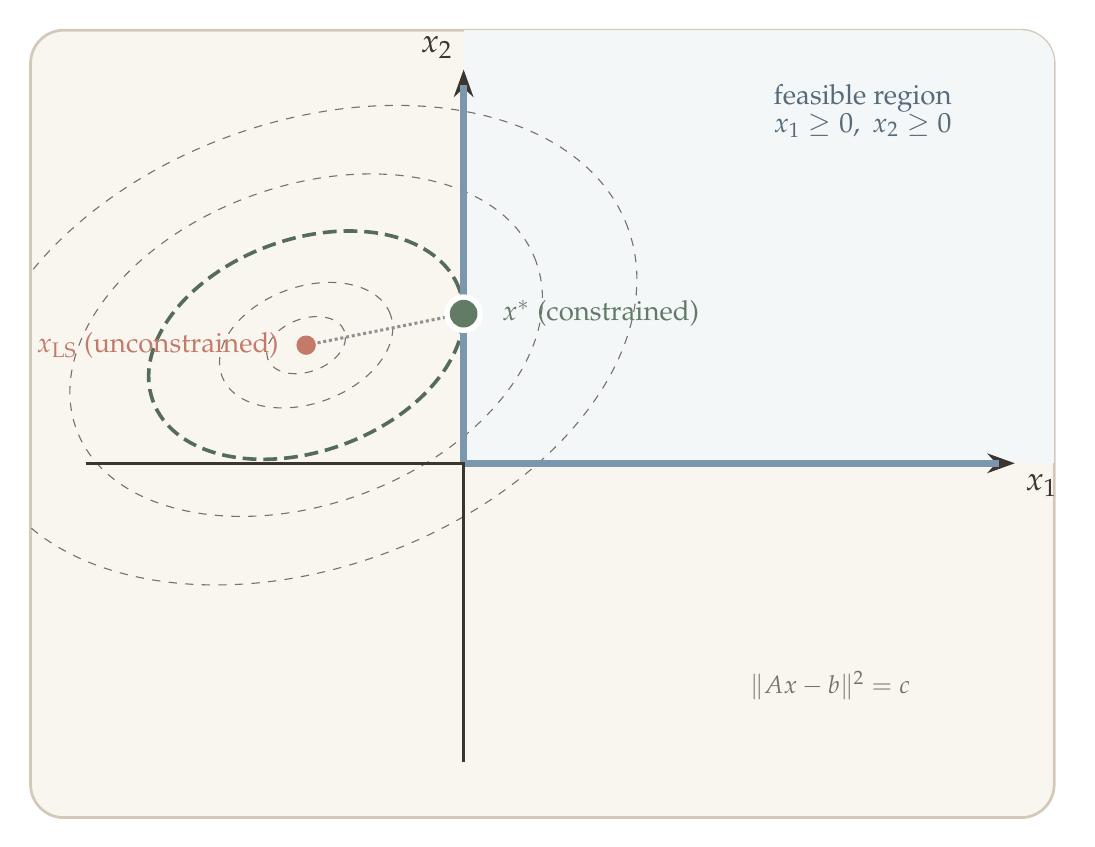
\begin{tikzpicture}[
  >={Stealth[length=3.5mm, width=2.5mm]},
  line width=1.2pt
]

% Background
\fill[cream, rounded corners=12pt] (-5.5,-4.5) rectangle (7.5,5.5);
\draw[border, line width=1pt, rounded corners=12pt] (-5.5,-4.5) rectangle (7.5,5.5);

% ── Key coordinates ──
% Unconstrained LS solution (infeasible, in the second quadrant)
\coordinate (xls) at (-2.0, 1.5);
% Constrained optimum: on the x2-axis (x1 = 0) at the exact tangent point
% of the critical contour ellipse.  Computed via tangent condition: (0, 1.898).
\coordinate (xstar) at (0, 1.9);

% ── Feasible region shading (first quadrant) ──
\begin{scope}
  \clip[rounded corners=12pt] (-5.5,-4.5) rectangle (7.5,5.5);
  \fill[stblue!8] (0,0) rectangle (7.5,5.5);
\end{scope}

% ── Contour ellipses of ||Ax - b||^2 ──
% Centre xls = (-2, 1.5), rotation 20 deg, aspect ratio b/a = 0.65.
% Critical tangent ellipse: a = 2.071, b = 1.346 (scale = 1).
\begin{scope}
  \clip[rounded corners=12pt] (-5.5,-4.5) rectangle (7.5,5.5);
  \begin{scope}[shift={(xls)}, rotate=20]
    % Inner contours (lie entirely in infeasible region)
    \draw[wmgray, thin, dashed] (0,0) ellipse (0.518 and 0.337);
    \draw[wmgray, thin, dashed] (0,0) ellipse (1.139 and 0.740);
    % Critical contour — tangent to x1 = 0 at xstar
    \draw[sage!70!black, line width=1.3pt, dash pattern=on 5pt off 2.5pt]
      (0,0) ellipse (2.071 and 1.346);
    % Outer contours (penetrate into feasible region)
    \draw[wmgray, thin, dashed] (0,0) ellipse (3.107 and 2.019);
    \draw[wmgray, thin, dashed] (0,0) ellipse (4.349 and 2.827);
  \end{scope}
\end{scope}

% ── Axes ──
\draw[->, dkbrown] (-4.8,0) -- (7.0,0);
\node[dkbrown, font=\large, anchor=north west] at (7.0,0) {$x_1$};
\draw[->, dkbrown] (0,-3.8) -- (0,5.0);
\node[dkbrown, font=\large, anchor=south east] at (0,5.0) {$x_2$};

% ── Feasible boundary emphasis (positive semi-axes, thicker blue) ──
\draw[stblue, line width=2.4pt] (0.02,0) -- (6.8,0);
\draw[stblue, line width=2.4pt] (0,0.02) -- (0,4.8);

% ── Feasible region label ──
\node[stblue!70!black, font=\normalsize, anchor=south west, align=center]
  at (3.8, 4.0) {feasible region\\[-2pt]$x_1\geq 0,\; x_2\geq 0$};

% ── Dotted projection line from xls to xstar ──
\draw[dkbrown!55, line width=1.1pt, densely dotted] (xls) -- (xstar);

% ── Unconstrained solution x_LS ──
\fill[terracotta] (xls) circle (3.5pt);
\node[terracotta, font=\normalsize, anchor=east, xshift=-6pt]
  at (xls) {$x_{\mathrm{LS}}$ (unconstrained)};

% ── Constrained optimum x* — drawn last so it sits on top of the axis ──
% White halo so the dot is clearly visible against the blue axis
\fill[white] (xstar) circle (7pt);
\fill[sage!80!black] (xstar) circle (5pt);
\node[sage!80!black, font=\normalsize, anchor=west, xshift=10pt]
  at (xstar) {$x^*$ (constrained)};

% ── Contour label ──
\node[wmgray, font=\small, anchor=north west]
  at (3.5, -2.5) {$\|Ax - b\|^2 = c$};

\end{tikzpicture}
\end{document}
